% Biên dịch: cd slides && tectonic tien_xu_ly.tex   (hoặc xelatex tien_xu_ly.tex)
\documentclass[aspectratio=169,11pt]{beamer}

\usepackage{fontspec}
\setsansfont{Arial}
\setmainfont{Arial}
\usepackage{graphicx}
\usepackage{booktabs}
\usepackage{tabularx}
\usepackage{array}
\usepackage{tikz}
\usetikzlibrary{positioning,arrows.meta}
\graphicspath{{../reports/figures/}}

% ---------- Giao diện tối giản ----------
\definecolor{ink}{HTML}{0B0B0B}
\definecolor{ink2}{HTML}{52514E}
\definecolor{muted}{HTML}{898781}
\definecolor{accent}{HTML}{2A78D6}
\definecolor{accentdark}{HTML}{1C5CAB}
\definecolor{wash}{HTML}{EEF4FC}
\definecolor{warn}{HTML}{E34948}
\definecolor{surface}{HTML}{FCFCFB}

\usetheme{default}
\setbeamercolor{background canvas}{bg=surface}
\setbeamercolor{normal text}{fg=ink}
\setbeamercolor{frametitle}{fg=ink,bg=}
\setbeamercolor{title}{fg=ink}
\setbeamercolor{subtitle}{fg=ink2}
\setbeamercolor{author}{fg=ink2}
\setbeamercolor{date}{fg=muted}
\setbeamercolor{structure}{fg=accent}
\setbeamercolor{itemize item}{fg=accent}
\setbeamercolor{itemize subitem}{fg=muted}
\setbeamercolor{block title}{fg=white,bg=accent}
\setbeamercolor{block body}{fg=ink,bg=wash}
\setbeamerfont{frametitle}{size=\Large,series=\bfseries}
\setbeamerfont{title}{size=\huge,series=\bfseries}
\setbeamertemplate{navigation symbols}{}
\setbeamertemplate{itemize items}[circle]
\setbeamertemplate{blocks}[rounded][shadow=false]
\setbeamertemplate{frametitle}{\vspace{0.6em}\insertframetitle\par\vspace{0.1em}{\color{accent}\rule{2.2em}{2pt}}}
\setbeamertemplate{footline}{\hfill{\color{muted}\footnotesize\insertframenumber/\inserttotalframenumber}\hspace{1.2em}\vspace{0.8em}}

\newcommand{\num}[1]{{\color{accentdark}\bfseries #1}}
\newcommand{\ghichu}[1]{{\color{muted}\footnotesize #1}}
\newcommand{\bignum}[2]{\begin{minipage}[t]{0.23\linewidth}\centering{\color{accentdark}\fontsize{26}{28}\selectfont\bfseries #1}\\[0.3em]{\small\color{ink2}#2}\end{minipage}}

\title{Thu thập \& Tiền xử lý dữ liệu\\Bất động sản TP.HCM từ Nhà Tốt}
\subtitle{Đồ án Data Science: Dự đoán giá \& Đánh giá cơ hội đầu tư}
\author{Họ tên học viên}
\date{25/09/2026}

\begin{document}

% ======================================================================
\begin{frame}[plain]
  \vspace{2em}
  \titlepage
\end{frame}

% ======================================================================
\begin{frame}{Kết quả chính}
  \vspace{1.5em}
  \centering
  \bignum{47.928}{tin thô, 22/22 quận}\hfill
  \bignum{43.490}{tin sạch sau tiền xử lý}\hfill
  \bignum{13}{tháng lịch sử giá theo phường}\hfill
  \bignum{0,87}{R\textsuperscript{2} kiểm tra nhanh (nhà ở)}

  \vspace{2.5em}
  \begin{itemize}
    \item 3 loại BĐS: \num{31.390} nhà ở · \num{6.217} căn hộ · \num{5.883} đất
    \item Bao phủ trọn bộ dữ liệu mẫu giảng viên cung cấp (3 quận, nhà ở) và có đủ các cột của mẫu
    \item Bàn giao: dataset sạch, 22 file theo quận, 3 bộ train/test sẵn sàng cho mô hình
  \end{itemize}
\end{frame}

% ======================================================================
\begin{frame}{Mục tiêu \& phạm vi}
  \begin{columns}[T]
    \begin{column}{0.5\linewidth}
      \textbf{Bài toán của đồ án}
      \begin{itemize}
        \item Dự đoán giá BĐS từ đặc điểm và vị trí
        \item Phát hiện tin bất thường, đánh giá khu vực / tin nên đầu tư
      \end{itemize}
      \vspace{0.8em}
      \textbf{Phần này đảm nhận}
      \begin{itemize}
        \item Thu thập dữ liệu (crawler)
        \item Tiền xử lý đến mức \emph{sẵn sàng cho mô hình}
      \end{itemize}
    \end{column}
    \begin{column}{0.5\linewidth}
      \textbf{Phạm vi dữ liệu}
      \begin{itemize}
        \item 22 quận/huyện TP.HCM \ghichu{(địa giới cũ, trước sáp nhập 07/2025)}
        \item Căn hộ, nhà ở, đất -- tin \emph{mua bán}
        \item Tin đang rao + tin đã gỡ / hết hạn
        \item Giữ cả tên phường cũ và phường mới
      \end{itemize}
      \vspace{0.8em}
      \begin{block}{Giới hạn nguồn}
        Tin trên Chợ Tốt chỉ tồn tại $\sim$60 ngày $\Rightarrow$ không lấy được tin 2 năm trước.
        Bù bằng \textbf{biểu đồ giá 13 tháng} + cào định kỳ.
      \end{block}
    \end{column}
  \end{columns}
\end{frame}

% ======================================================================
\begin{frame}{Pipeline}
  \centering
  \vspace{0.5em}
  \begin{tikzpicture}[
      box/.style={draw=accent, fill=wash, rounded corners=3pt, align=center, minimum height=1.25cm,
                  text width=2.25cm, font=\small},
      outbox/.style={draw=muted, fill=white, rounded corners=3pt, align=center, text width=2.6cm, font=\footnotesize},
      arr/.style={-{Stealth[length=2.2mm]}, accent, thick}]
    \node[box] (a) {API Chợ Tốt\\22 quận};
    \node[box, right=0.45cm of a] (b) {Trích xuất\\giải mã nhãn};
    \node[box, right=0.45cm of b] (c) {Làm sạch\\loại dòng};
    \node[box, right=0.45cm of c] (d) {Sửa ô\\+ đặc trưng};
    \node[box, right=0.45cm of d] (e) {Chuẩn bị\\mô hình};
    \node[box, below=0.7cm of a] (m) {API biểu đồ giá\\13 tháng};
    \draw[arr] (a) -- (b); \draw[arr] (b) -- (c); \draw[arr] (c) -- (d); \draw[arr] (d) -- (e);
    \draw[arr] (m) -| (d);
    \node[outbox, below=1.9cm of c] (o1) {\texttt{rejected\_rows.csv}\\lý do từng dòng};
    \node[outbox, below=1.9cm of d] (o2) {\texttt{clean.csv / .parquet}\\\texttt{by\_district/}, \texttt{dinh\_dang\_mau/}};
    \node[outbox, below=1.9cm of e] (o3) {\texttt{model\_ready/}\\train / test / encoder};
    \draw[muted, dashed] (c) -- (o1); \draw[muted, dashed] (d) -- (o2); \draw[muted, dashed] (e) -- (o3);
  \end{tikzpicture}

  \vspace{0.6em}
  \ghichu{Mỗi lần cào lưu vào \texttt{data/raw/<run\_id>/} kèm \texttt{manifest.json}; nhật ký các lần cào: \texttt{data/history/snapshots.csv.gz}}
\end{frame}

% ======================================================================
\begin{frame}{Thu thập dữ liệu}
  \begin{columns}[T]
    \begin{column}{0.55\linewidth}
      \small
      \textbf{Tin rao} \ghichu{(API \texttt{ad-listing})}
      \begin{itemize}
        \item Theo từng quận, 50 tin/trang, hết mọi trang
        \item Thêm tin đã gỡ $\Rightarrow$ \num{gần gấp đôi} (24,7 $\to$ 47,9 nghìn)
        \item Retry, thử lại trang lỗi, \texttt{manifest.json}
      \end{itemize}
      \vspace{0.5em}
      \textbf{Biểu đồ giá} \ghichu{(API \texttt{market-price/charts})}
      \begin{itemize}
        \item Đơn giá trung vị theo tháng, 13 tháng, theo phường × loại BĐS × phân nhóm
        \item 792 biểu đồ, gắn cho \num{99,8\%} số tin
      \end{itemize}
    \end{column}
    \begin{column}{0.42\linewidth}
      \begin{block}{Đối chiếu bộ dữ liệu mẫu}
        \small
        \begin{tabular}{@{}lrr@{}}
          Nhà ở & Mẫu & Dataset này \\ \midrule
          Gò Vấp & 4.374 & 3.404 \\
          Bình Thạnh & 2.665 & 1.921 \\
          Phú Nhuận & 1.234 & 908 \\
        \end{tabular}\\[0.4em]
        \footnotesize Ít dòng hơn vì đã loại tin trùng; riêng file mẫu Gò Vấp có 216 tiêu đề trùng và 4,5\% dòng trống.\\[0.3em]
        Có đủ 22/23 cột của mẫu. \textbf{Không thu thập số điện thoại} (dữ liệu cá nhân).
      \end{block}
    \end{column}
  \end{columns}
\end{frame}

% ======================================================================
\begin{frame}{Lỗi phát hiện \& đã sửa trong code ban đầu}
  \small
  \begin{tabularx}{\linewidth}{@{}p{3.6cm}X X@{}}
    \toprule
    \textbf{Vấn đề} & \textbf{Hậu quả} & \textbf{Cách sửa} \\ \midrule
    Mã pháp lý dịch sai & Mã 6 = ``Sổ hồng riêng'' (căn hộ) bị ghi ``Chưa xác định'' & Dùng nhãn chữ của API, bảng mã tách theo loại BĐS \\
    Gộp nhà, căn hộ, đất khi so giá & Đơn giá/m\textsuperscript{2} khác bản chất, ngoại lai sai & Ngưỡng + nhóm tham chiếu theo quận × loại BĐS \\
    Ngưỡng đơn giá chung 5 tr/m\textsuperscript{2} & Loại oan $\sim$11\% tin đất (Củ Chi) & Ngưỡng riêng: đất 0,2 tr/m\textsuperscript{2} \\
    Điền thiếu trước khi chia train/test & Rò rỉ dữ liệu; đất bị điền số phòng ngủ & Giữ NaN + cờ thiếu; điền thiếu fit trên train \\
    Lỗi mạng trả trang rỗng & Mất phần còn lại của quận, không báo & Retry, thử lại trang lỗi, manifest \\
    Bộ lọc ``2 năm'' & Không có tác dụng (tin chỉ sống 60 ngày) & Tin đã gỡ + biểu đồ giá 13 tháng \\
    \bottomrule
  \end{tabularx}
\end{frame}

% ======================================================================
\begin{frame}{Làm sạch: loại 4.438 dòng (9,3\%)}
  \centering
  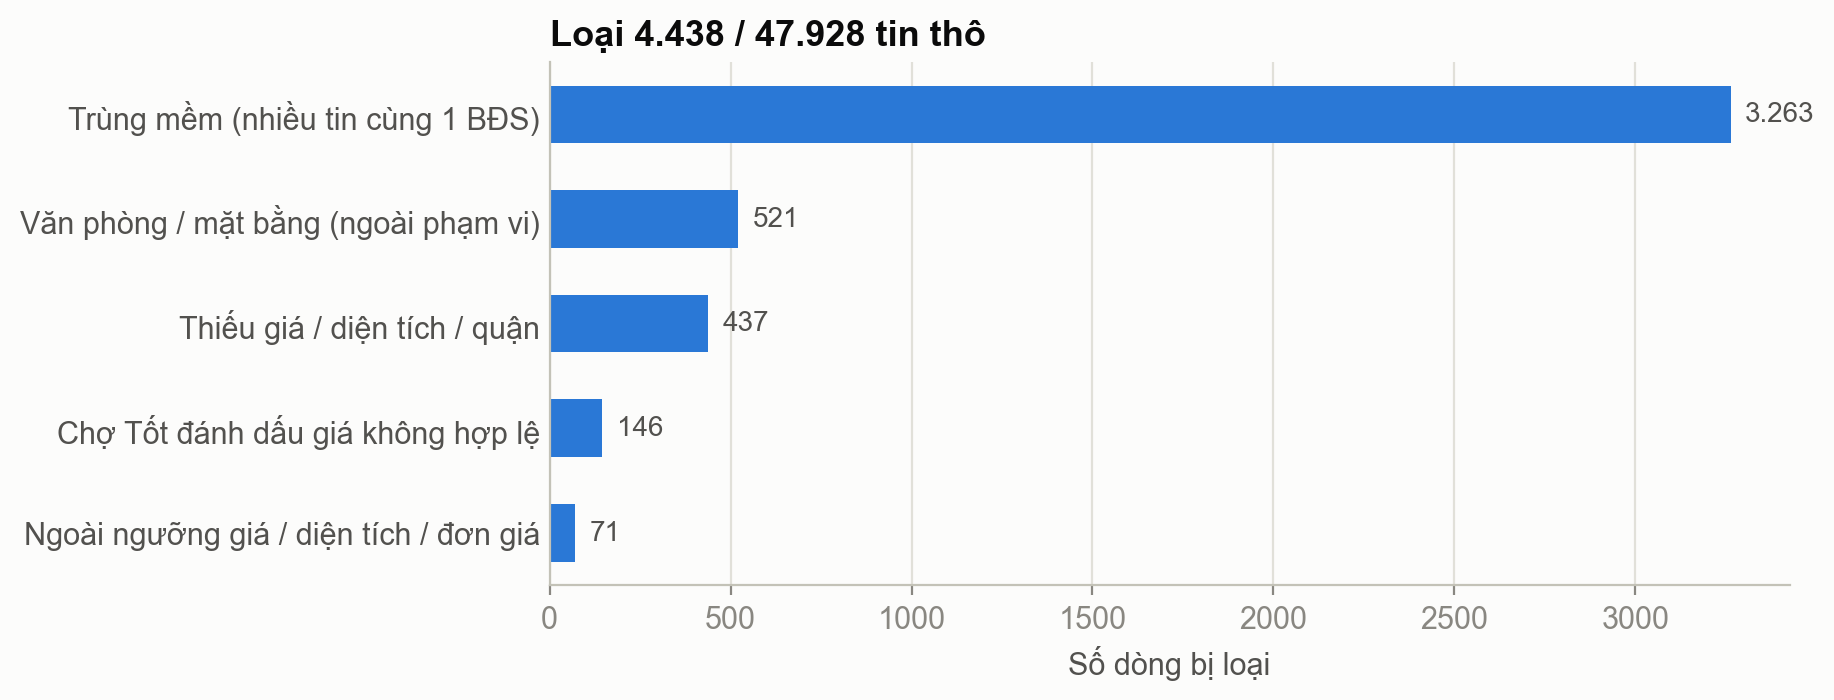
\includegraphics[width=0.78\linewidth]{01_rejections.png}

  \small
  \begin{columns}[T]
    \begin{column}{0.48\linewidth}
      \begin{itemize}
        \item \textbf{Trùng mềm}: cùng loại, phường, giá, diện tích, số phòng, số tầng $\to$ giữ tin sớm nhất; số bản trùng thành biến \texttt{n\_duplicate\_posts}
      \end{itemize}
    \end{column}
    \begin{column}{0.48\linewidth}
      \begin{itemize}
        \item Ngưỡng \textbf{riêng cho từng loại BĐS}
        \item Dòng bị loại lưu kèm lý do: \texttt{rejected\_rows.csv}
      \end{itemize}
    \end{column}
  \end{columns}
\end{frame}

% ======================================================================
\begin{frame}{Sửa từng ô: đặt NaN thay vì loại cả dòng}
  \begin{columns}[T]
    \begin{column}{0.5\linewidth}
      \footnotesize
      \begin{tabular}{@{}lr@{}}
        \toprule
        Giá trị phi lý & Số dòng \\ \midrule
        Tọa độ ngoài TP.HCM & 63 \\
        Chiều ngang $\le 0$ hoặc $> 50$ m & 100 \\
        Chiều dài $\le 0$ hoặc $> 200$ m & 17 \\
        Căn hộ $> 6$ phòng ngủ & 54 \\
        Nhà ở $> 10$ tầng & 49 \\
        Số WC $>$ số phòng ngủ + 5 & 42 \\ \midrule
        DT lệch ngang × dài $> 2$ lần \ghichu{(gắn cờ)} & 472 \\
        \bottomrule
      \end{tabular}
    \end{column}
    \begin{column}{0.46\linewidth}
      \begin{block}{Tọa độ chỉ ở mức đường / phường}
        \small
        Chợ Tốt không trả vị trí thật của căn nhà:
        \begin{itemize}
          \item \num{32.061} tin: tâm con đường
          \item \num{11.366} tin: tâm phường (1 điểm dùng chung cho nhiều đường)
        \end{itemize}
        $\Rightarrow$ biến \texttt{geo\_precision}; không nên tính khoảng cách tới tiện ích ở mức mét.
      \end{block}
    \end{column}
  \end{columns}
\end{frame}

% ======================================================================
\begin{frame}{Dữ liệu thiếu}
  \begin{columns}[c]
    \begin{column}{0.58\linewidth}
      \centering
      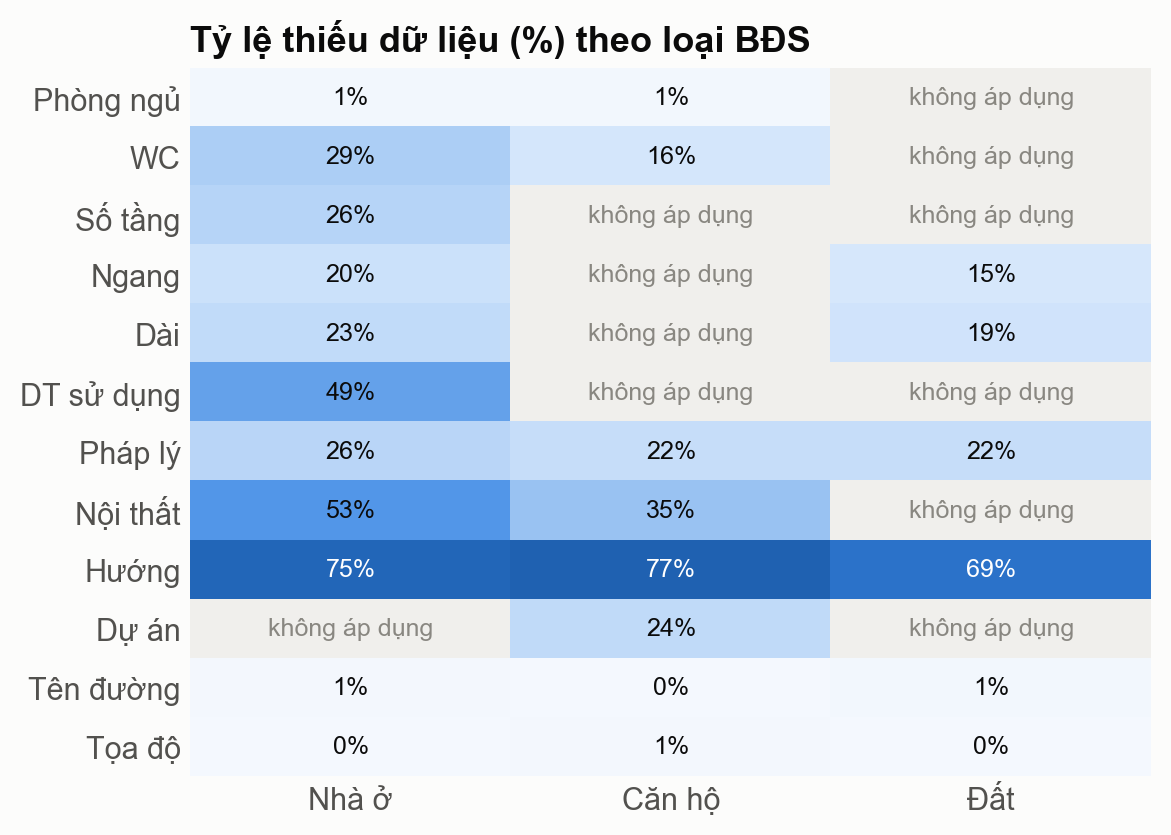
\includegraphics[width=\linewidth]{02_missing.png}
    \end{column}
    \begin{column}{0.4\linewidth}
      \small
      \begin{itemize}
        \item \textbf{``Không áp dụng'' $\neq$ thiếu}: đất không có phòng ngủ, căn hộ không có số tầng nhà $\to$ để NaN, không điền
        \item Hướng nhà thiếu $\sim$75\%, nội thất thiếu 35--53\%
        \item Ở bước làm sạch: \textbf{không điền}, chỉ thêm cờ \texttt{*\_missing}
        \item Điền trung vị / ``missing'' \textbf{chỉ fit trên train}
      \end{itemize}
    \end{column}
  \end{columns}
\end{frame}

% ======================================================================
\begin{frame}{Phân phối giá}
  \centering
  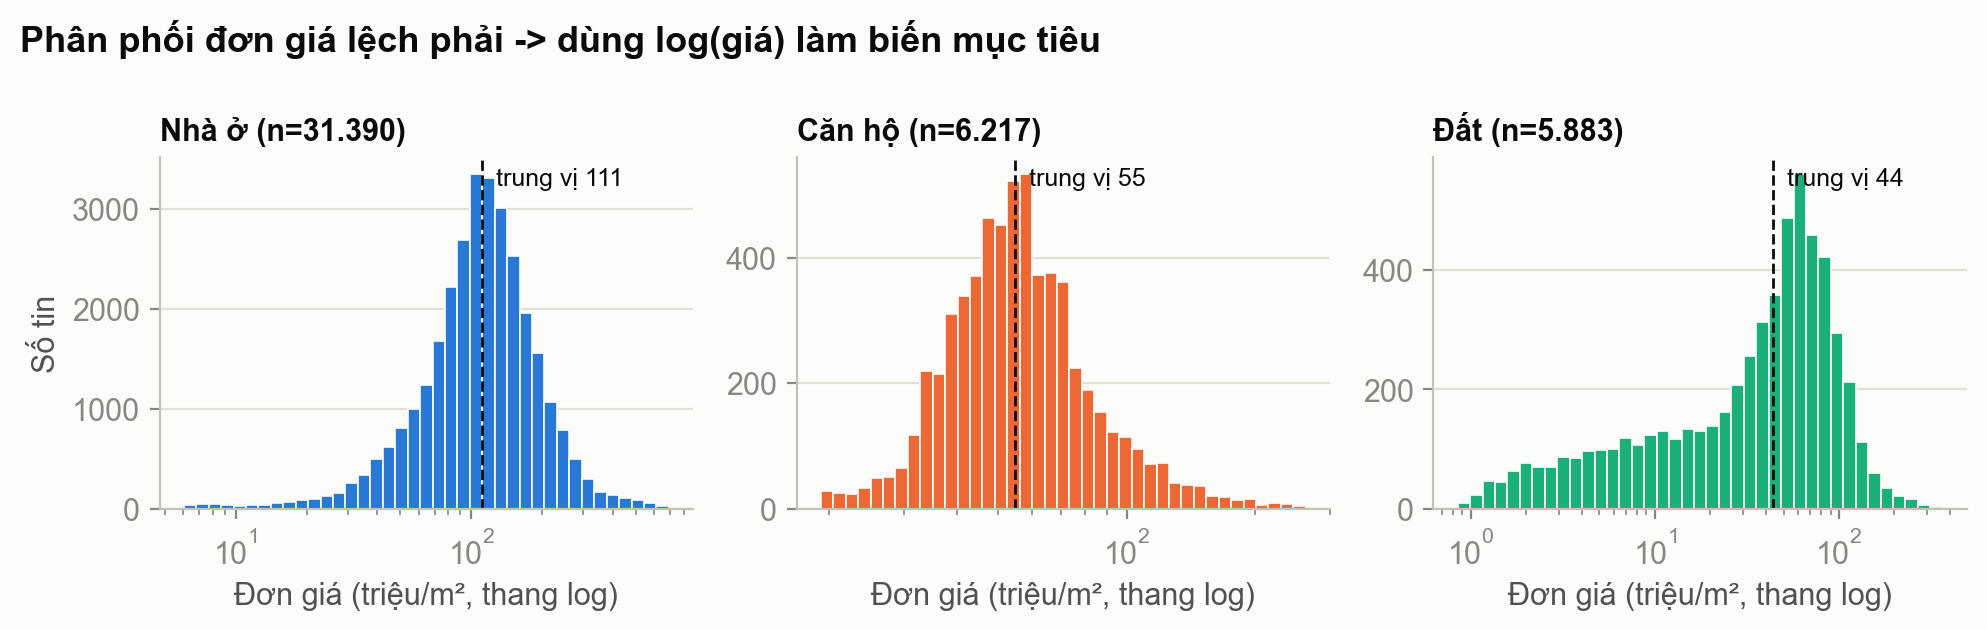
\includegraphics[width=\linewidth]{03_price_distribution.png}

  \vspace{0.3em}
  \small
  \begin{itemize}
    \item Đơn giá lệch phải mạnh $\Rightarrow$ biến mục tiêu \texttt{target\_log\_price} = ln(giá tỷ đồng)
    \item Đất có \textbf{hai đỉnh}: đất nông nghiệp ($\sim$1--10 tr/m\textsuperscript{2}) và thổ cư ($\sim$50--100 tr/m\textsuperscript{2}) $\Rightarrow$ \texttt{land\_type} là biến bắt buộc
  \end{itemize}
\end{frame}

% ======================================================================
\begin{frame}{Đặc trưng bổ sung}
  \begin{columns}[T]
    \begin{column}{0.47\linewidth}
      \small
      \textbf{Có cấu trúc (thay cho dò từ khóa)}
      \begin{itemize}
        \item \texttt{char\_*}: mặt tiền, hẻm xe hơi, nở hậu, quy hoạch, thổ cư\dots
        \item Nội thất, loại đất / căn hộ, dự án, phường mới
      \end{itemize}
      \textbf{Giá khu vực}
      \begin{itemize}
        \item \texttt{bieu\_do\_gia} (13 giá trị), tăng giá theo năm, tăng giá làm mượt
      \end{itemize}
      \textbf{Giá thuê trích từ mô tả}
      \begin{itemize}
        \item ``cho thuê 40tr/tháng'' $\to$ tỷ suất gộp: \num{2.994} tin, trung vị \num{3,0\%/năm}
      \end{itemize}
    \end{column}
    \begin{column}{0.52\linewidth}
      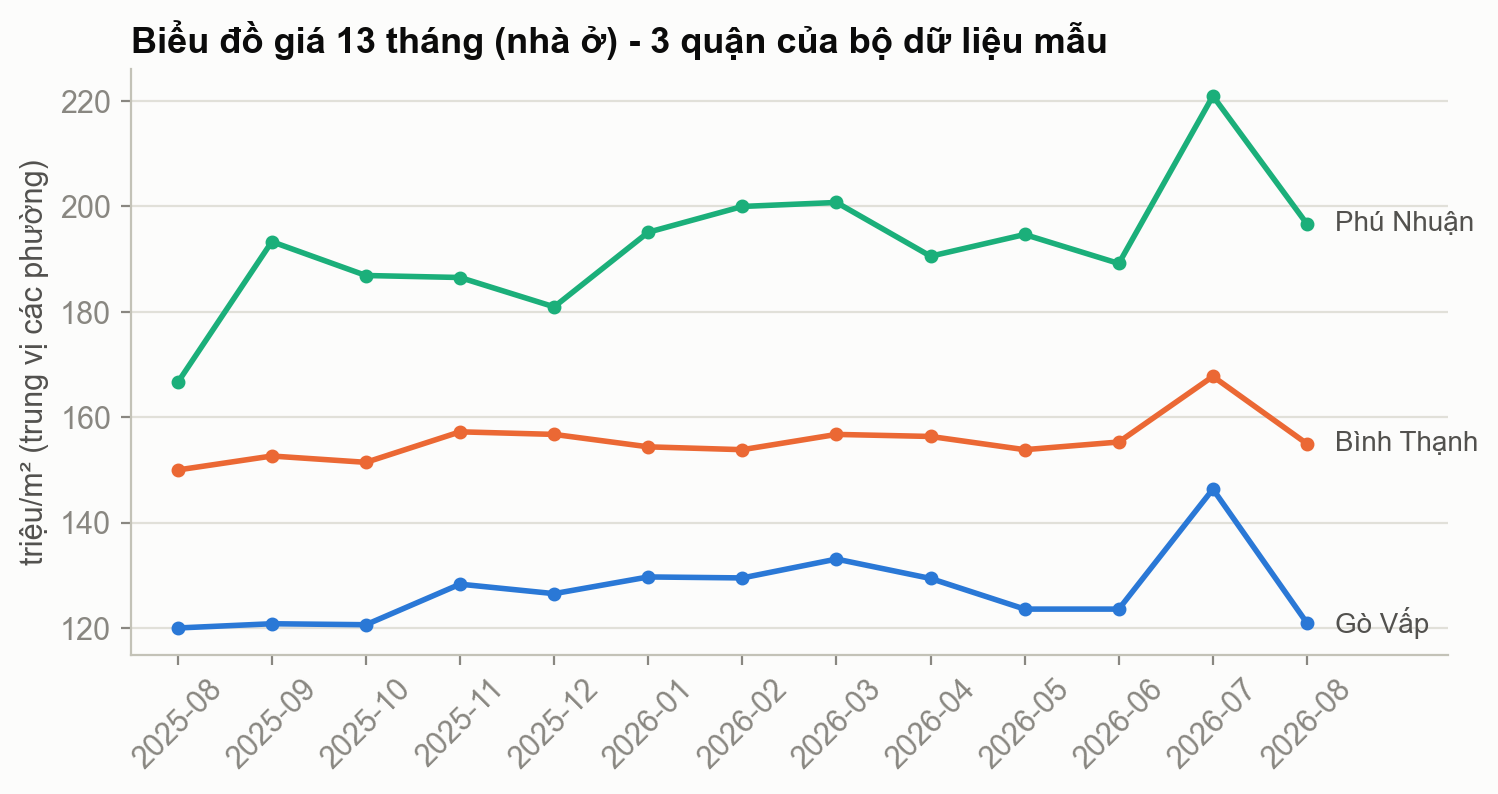
\includegraphics[width=\linewidth]{06_market_trend.png}
      \ghichu{Biểu đồ giá cấp phường còn nhiễu theo tháng $\to$ nên làm mượt hoặc gộp lên cấp quận.}
    \end{column}
  \end{columns}
\end{frame}

% ======================================================================
\begin{frame}{EDA: đơn giá nhà ở theo quận}
  \begin{columns}[c]
    \begin{column}{0.58\linewidth}
      \centering
      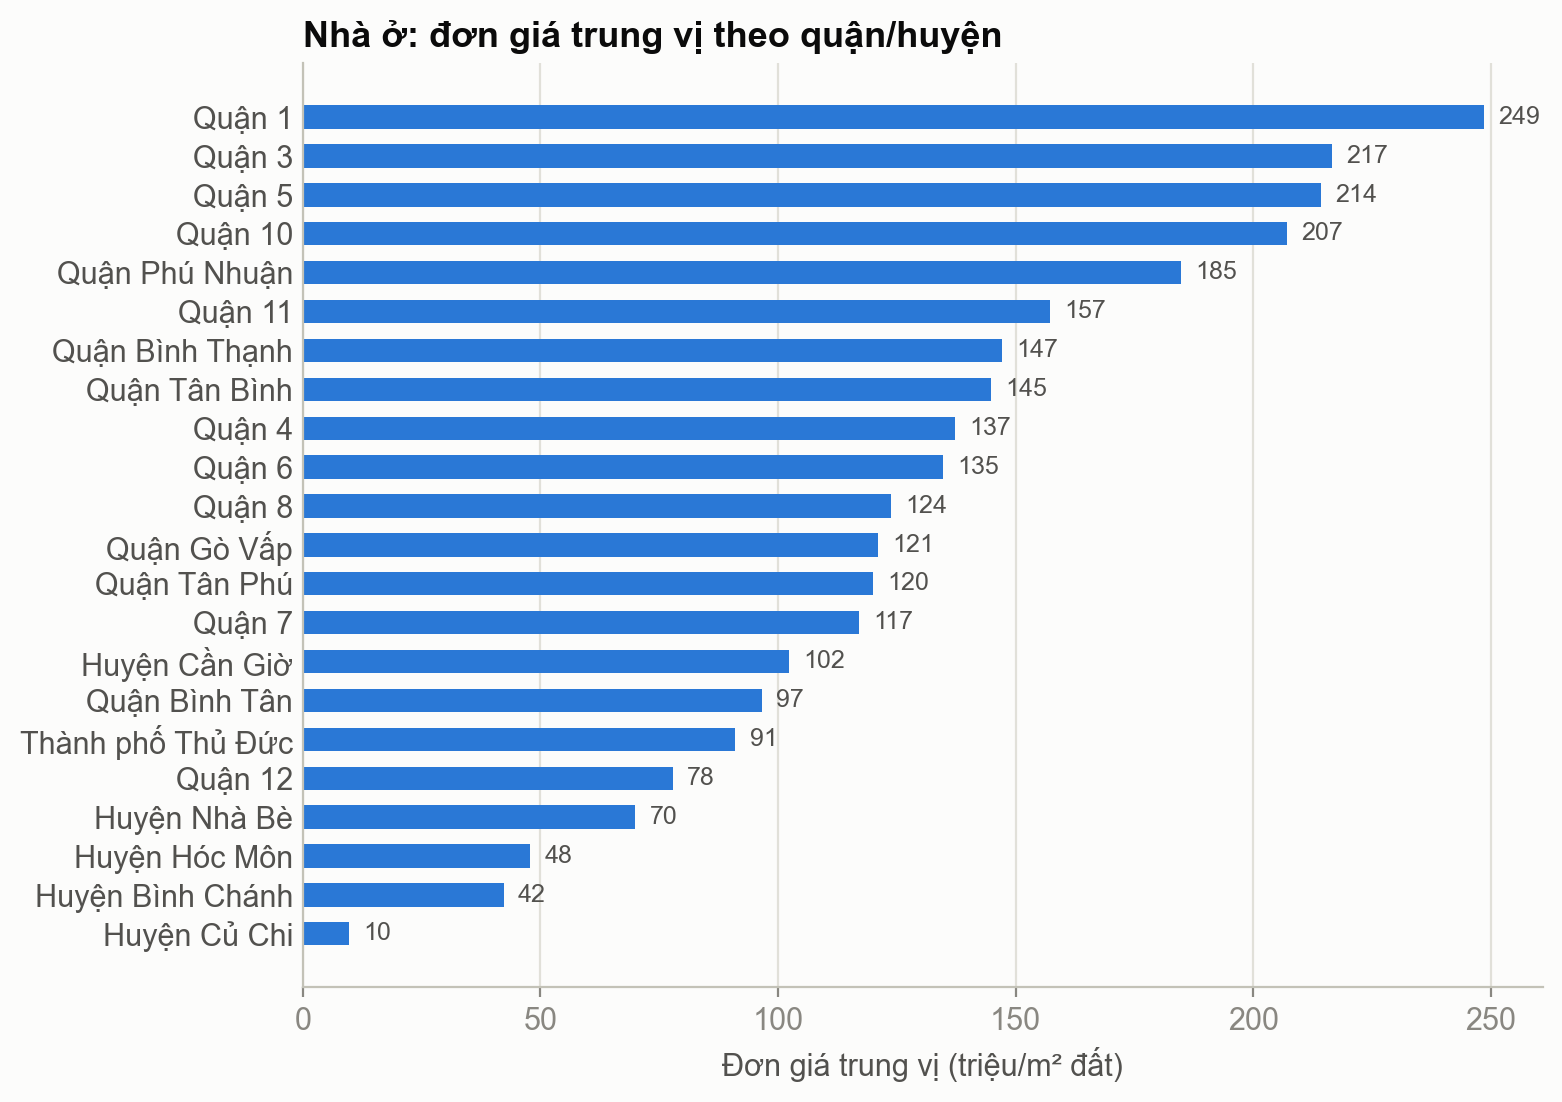
\includegraphics[height=0.8\textheight]{04_district_price_nha_o.png}
    \end{column}
    \begin{column}{0.4\linewidth}
      \small
      \begin{itemize}
        \item Chênh lệch trên 20 lần giữa trung tâm (Q1 $\sim$250 tr/m\textsuperscript{2}) và Củ Chi ($\sim$10 tr/m\textsuperscript{2})
        \item $\Rightarrow$ vị trí (quận, phường, đường) là nhóm biến quan trọng nhất
        \item Phường / đường / dự án có hàng nghìn giá trị $\to$ \textbf{Target Encoding}
      \end{itemize}
    \end{column}
  \end{columns}
\end{frame}

% ======================================================================
\begin{frame}{EDA: tín hiệu đầu tư theo quận}
  \centering
  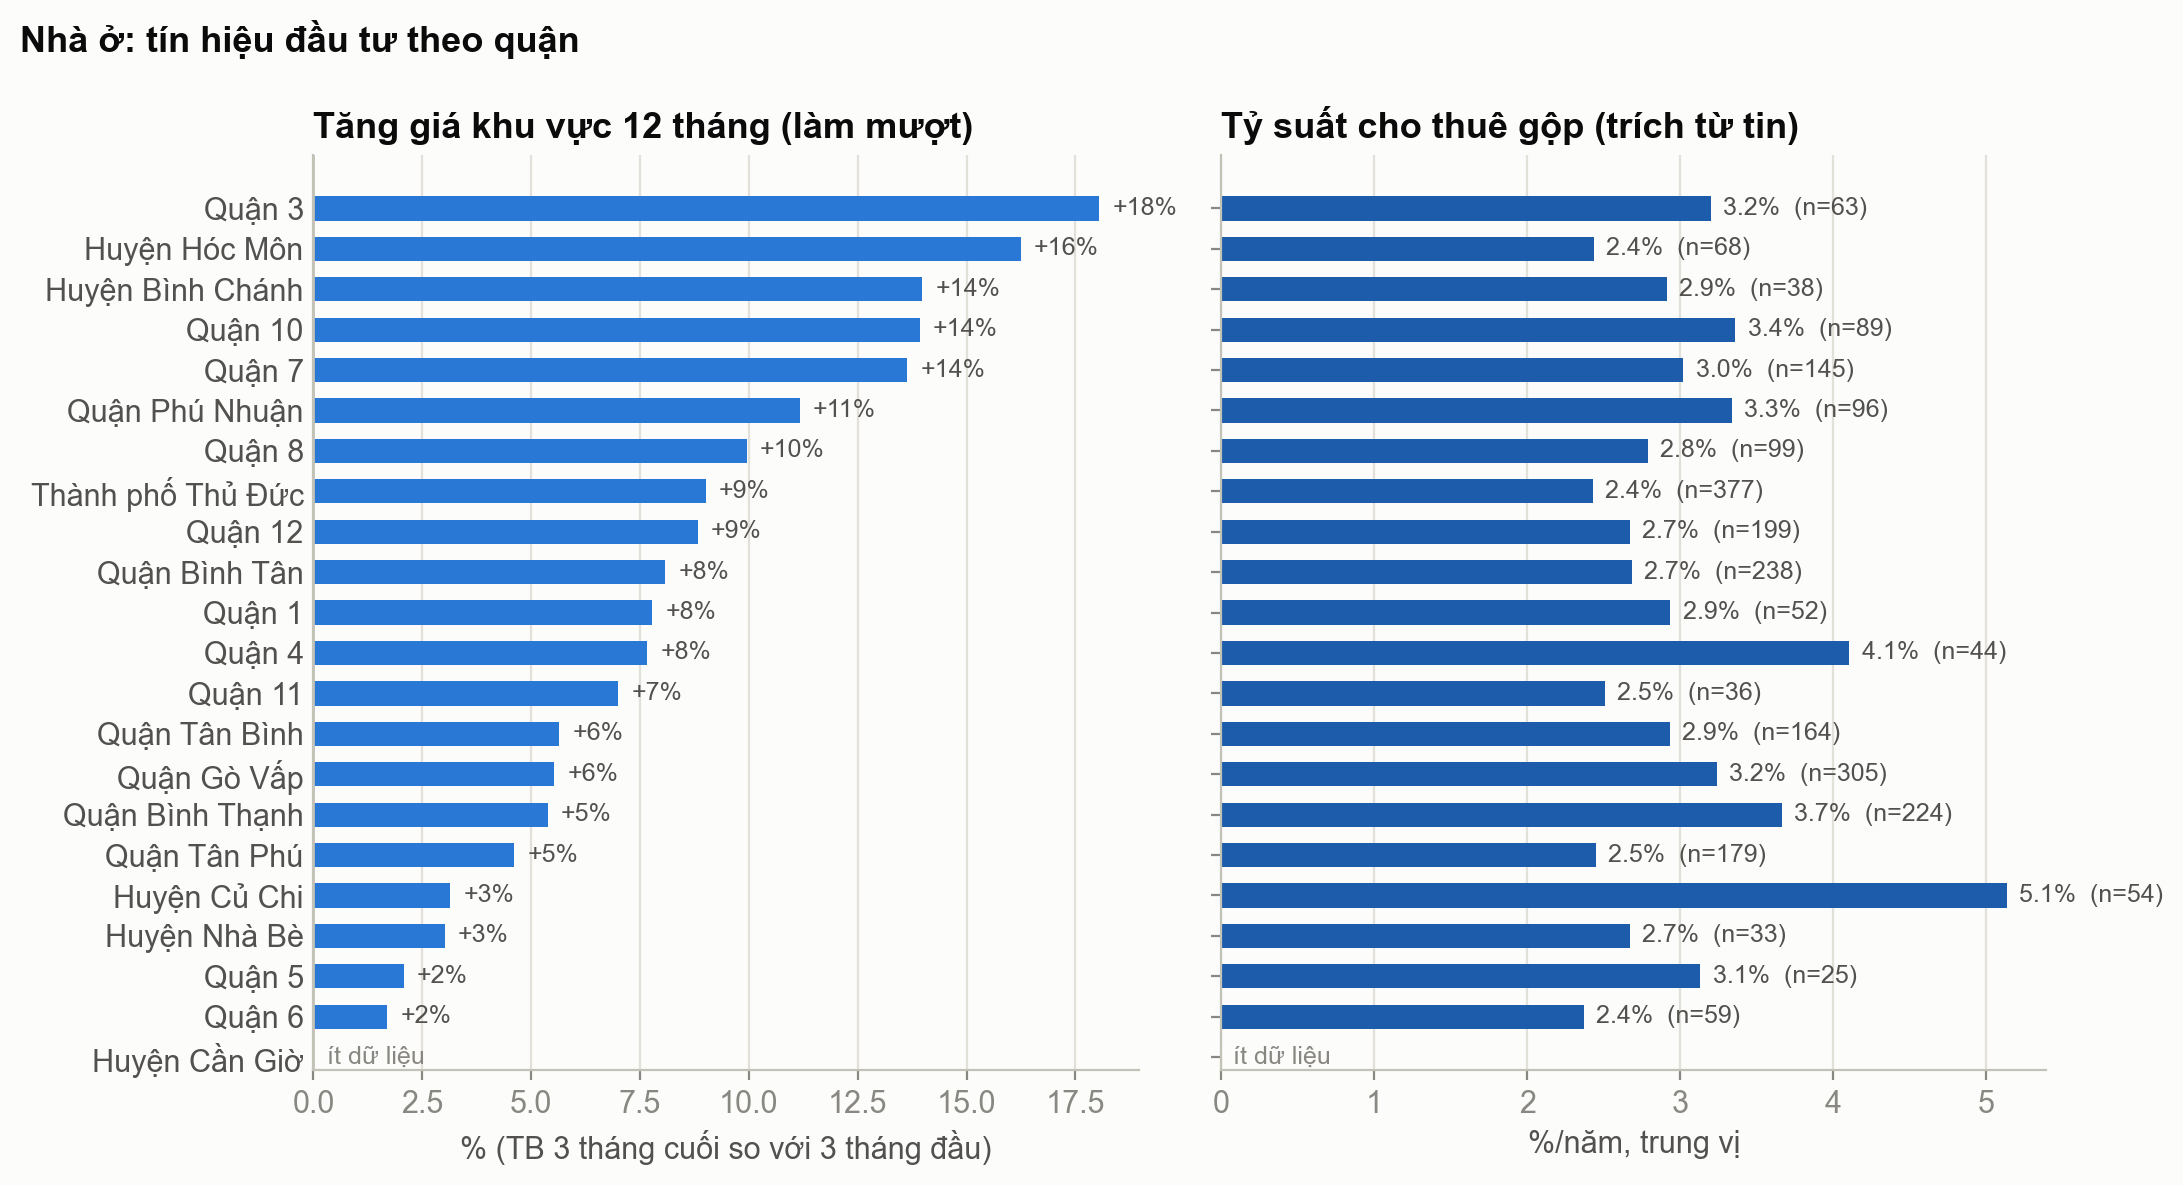
\includegraphics[height=0.74\textheight]{05_growth_yield_nha_o.png}

  \ghichu{Ẩn quận có ít hơn 100 tin (tăng giá) hoặc ít hơn 15 tin có giá thuê (tỷ suất) vì quá nhiễu. Đây là số liệu mô tả, chưa phải khuyến nghị đầu tư.}
\end{frame}

% ======================================================================
\begin{frame}{Chuẩn bị dữ liệu cho mô hình}
  \begin{columns}[T]
    \begin{column}{0.52\linewidth}
      \small
      \begin{enumerate}
        \item \textbf{Mỗi loại BĐS một bộ} train/test riêng
        \item \textbf{Chia 80/20 theo người đăng} (\texttt{account\_id}): tin của cùng một môi giới rất giống nhau $\to$ nếu nằm ở cả hai tập thì đánh giá đẹp giả
        \item \textbf{Loại ngoại lai chỉ trên train} (3×IQR log đơn giá theo quận): 8 / 89 / 45 tin
        \item \textbf{Fit trên train, áp dụng cho test}:
          \begin{itemize}
            \item số: trung vị + chuẩn hóa
            \item phân loại: One-Hot (gộp nhóm $<20$)
            \item phường / đường / dự án: Target Encoding cross-fitting
          \end{itemize}
      \end{enumerate}
    \end{column}
    \begin{column}{0.46\linewidth}
      \begin{block}{Không dùng làm biến đầu vào}
        \small
        \textbf{Rò rỉ nhãn} (tính từ chính giá):\\
        đơn giá/m\textsuperscript{2}, độ lệch so với trung vị, cờ ngoại lai / cơ hội đầu tư, giá thuê nêu trong tin\\[0.4em]
        \textbf{Chỉ biết sau khi đăng}:\\
        số ngày đăng, đã gỡ, đã đẩy tin
      \end{block}
      \vspace{0.3em}
      \footnotesize
      \begin{tabular}{@{}lrrr@{}}
        \toprule
         & Train & Test & Biến \\ \midrule
        Căn hộ & 4.956 & 1.253 & 89 \\
        Nhà ở & 25.214 & 6.087 & 95 \\
        Đất & 4.718 & 1.120 & 73 \\
        \bottomrule
      \end{tabular}
    \end{column}
  \end{columns}
\end{frame}

% ======================================================================
\begin{frame}{Kiểm tra nhanh: dữ liệu có đủ thông tin?}
  \begin{columns}[c]
    \begin{column}{0.55\linewidth}
      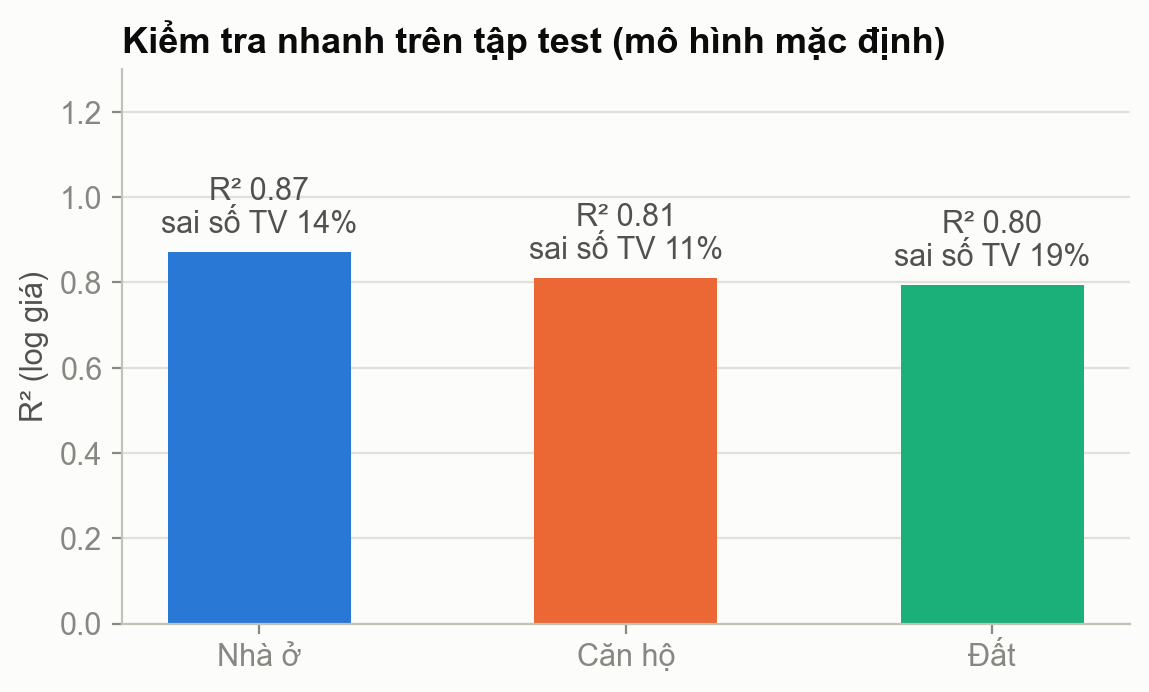
\includegraphics[width=\linewidth]{07_baseline.png}
    \end{column}
    \begin{column}{0.43\linewidth}
      \small
      \begin{itemize}
        \item \texttt{HistGradientBoosting} mặc định, \textbf{không tinh chỉnh}, đánh giá trên tập test
        \item Sai số giá trung vị: 11\% (căn hộ), 14\% (nhà ở), 19\% (đất)
        \item Đất khó nhất: MAPE 45\% do phân khúc nông nghiệp giá rất thấp
        \item Mục đích: xác nhận dữ liệu dùng được, \emph{không phải} kết quả mô hình cuối
      \end{itemize}
    \end{column}
  \end{columns}
\end{frame}

% ======================================================================
\begin{frame}{Hạn chế \& bước tiếp theo}
  \begin{columns}[T]
    \begin{column}{0.5\linewidth}
      \textbf{Hạn chế}
      \small
      \begin{itemize}
        \item Giá rao $\neq$ giá giao dịch
        \item Tin đã gỡ $\neq$ đã bán (có thể chỉ hết hạn)
        \item Tọa độ chỉ ở mức đường / phường
        \item Biểu đồ giá phường nhiễu khi ít tin
        \item Cờ ``cơ hội đầu tư'' theo luật còn thô (20\% số tin)
        \item Phạm vi TP.HCM cũ, chưa gồm Bình Dương, Bà Rịa - Vũng Tàu
      \end{itemize}
    \end{column}
    \begin{column}{0.5\linewidth}
      \textbf{Bước tiếp theo}
      \small
      \begin{itemize}
        \item Cào lại hàng tuần để tích lũy chuỗi thời gian
        \item Mô hình giá theo từng loại BĐS (GBM, tinh chỉnh)
        \item Cơ hội đầu tư = \textbf{phần dư mô hình} (giá rao thấp hơn giá dự đoán), kết hợp tăng giá khu vực và tỷ suất cho thuê
        \item Phát hiện bất thường: Isolation Forest trên phần dư
      \end{itemize}
    \end{column}
  \end{columns}
\end{frame}

% ======================================================================
\begin{frame}{Sản phẩm bàn giao}
  \footnotesize
  \renewcommand{\arraystretch}{1.15}
  \begin{tabularx}{\linewidth}{@{}>{\ttfamily}p{0.52\linewidth}X@{}}
    \toprule
    \texttt{data/processed/nhatot\_tphcm\_clean.csv / .parquet} & Dataset sạch, 43.490 dòng, 116 cột \\
    \texttt{data/processed/by\_district/}, \texttt{by\_property\_type/} & Chia theo 22 quận / 3 loại BĐS \\
    \texttt{data/processed/dinh\_dang\_mau/} & Đúng tên cột của bộ dữ liệu mẫu \\
    \texttt{data/processed/market\_price\_monthly.csv} & Giá khu vực theo tháng (13 tháng) \\
    \texttt{data/processed/rejected\_rows.csv} & Dòng bị loại + lý do \\
    \texttt{data/model\_ready/<loại>/} & train / test, \texttt{preprocessor.joblib}, \texttt{features.json} \\
    \texttt{reports/} & Thống kê theo quận, tỷ lệ thiếu, biểu đồ \\
    \texttt{GHI\_CHU\_TIEN\_XU\_LY.md} & Nhật ký quyết định tiền xử lý \\
    \texttt{BAO\_CAO\_TIEN\_XU\_LY.md} & Danh mục biến \\
    \bottomrule
  \end{tabularx}

  \vspace{1em}
  Chạy lại toàn bộ: \texttt{python run\_pipeline.py} \ghichu{($\sim$30 phút)}
\end{frame}

\end{document}
